\section{Data Communication Directives}

\subsection{{\bf shadow} Directive / {\bf reflect} Construct}

The stencil computation frequently appears in scientific computations,
where array elements a[i-1] and a[i+1] are referenced to update a[i]. If
a[i] is on the boundary area of a distributed array on a node, a[i+1]
may reside on another node.

Because it costs largely to copy a[i+1] from the neighboring node to
update each a[i], a technique of copying collectively elements on the
neighboring node to the area added to the distributed array on each node
is usually adopted. In XMP, such additional region is called “shadow.”

\subsubsection{Declare Shadow}

\paragraph{Widths of lower/upper bounds are the same}

Shadow areas can be declared with the shadow directive. In the example
below, an array a has shadow areas of size one on both the lower and
upper bounds.

\begin{XCexample}
#pragma xmp nodes p[4]
#pragma xmp template t[16]
#pragma xmp distribute t[block] onto p
double a[16];
#pragma xmp align a[i] with t[i]
#pragma xmp shadow a[1]
\end{XCexample}

\begin{XFexample}
!$xmp nodes p(4)
!$xmp template t(16)
!$xmp distribute t(block) onto p
real :: a(16)
!$xmp align a(i) with t(i)
!$xmp shadow a(1)
\end{XFexample}

\begin{figure}
  \centering
  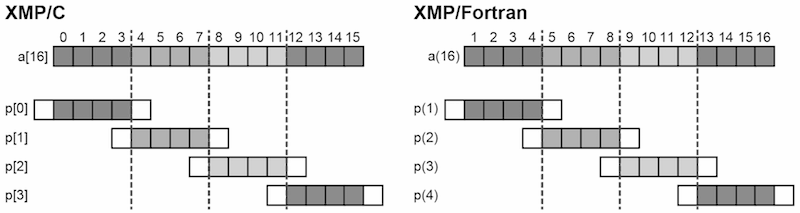
\includegraphics{figs/shadow.png}
\end{figure}

In the figure above, colored elements are those that each node owns and white ones are shadow.

\begin{mynote}
Distributed arrays in a cyclic manner cannot have shadow.  
\end{mynote}

\paragraph{Widths of lower/upper bounds are different}

For some programs, it is natural that the widths of the shadow area on
the lower and upper bounds are different. There is also a case where the
shadow area exists only on either of the bounds. In the example below,
it is declared that a distributed array a has a shadow area of width one
only on the upper bound.

\begin{XCexample}
#pragma xmp nodes p[4]
#pragma xmp template t[16]
#pragma xmp distribute t(block) onto p
double a[16];
#pragma xmp align a[i] with t[i]
#pragma xmp shadow a[0:1]
\end{XCexample}

\begin{XFexample}
!$xmp nodes p(4)
!$xmp template t(16)
!$xmp distribute t(block) onto p
real :: a(16)
!$xmp align a(i) with t(i)
!$xmp shadow a(0:1)
\end{XFexample}

\begin{figure}
  \centering
  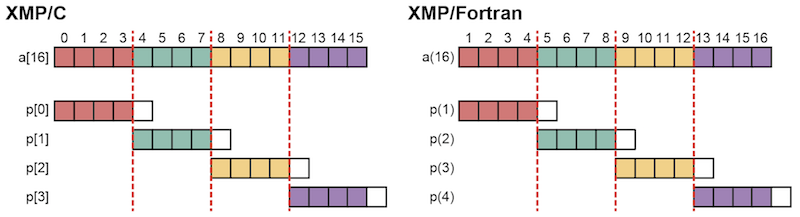
\includegraphics{figs/shadow_uneven.png}
\end{figure}

The values on the left- and right-hand sides of a colon designate the
widths on the lower and upper bounds, respectively.

\subsubsection{Update Shadow}

\paragraph{General}

To copy data to shadow areas from neighboring nodes, use the reflect
directive. In the example below, an array a having shadow areas of width
one on each the upper and lower bounds is reflected.

\begin{XCexample}
#pragma xmp reflect (a)

#pragma xmp loop on t[i]
for(int i=1;i<15;i++)
  a[i] = (a[i-1] + a[i] + a[i+1])/3;
\end{XCexample}

\begin{XFexample}
!$xmp reflect (a)

!xmp loop on t(i)
do i=2, 15
  a(i) = (a(i-1) + a(i) + a(i+1))/3
enddo
\end{XFexample}

\begin{figure}
  \centering
  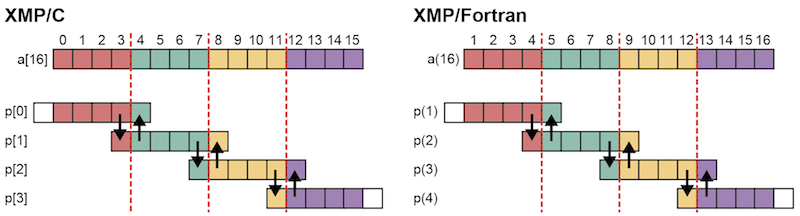
\includegraphics{figs/reflect.png}
\end{figure}

With this reflect directive, in XMP/C, node p[1] sends an element a[4]
to the shadow area on the upper bound on node p[0] and a[7] to the
shadow area on the lower bound on p[2]; p[0] sends an element a[3] to
the shadow area on the lower bound on p[1], and p[2] sends a[8] to the
shadow area on the upper bound on p[1].

Similarly, in XMP/Fortran, node p(2) sends an element a(5) to the shadow
area on the upper bound on node p(1) and a(8) to the shadow area on the
lower bound on p(3); p(1) sends an element a(4) to the shadow area on
the lower bound on p(2), and p(3) sends a(9) to the shadow area on the
upper bound on p(2).

\paragraph{Specify Width}

The default behavior of a reflect directive is to update the whole of
the shadow area declared by a shadow directive. However, there are some
cases where a specific part of the shadow area is to be updated to
reduce the communication size in a point of the code.

To update only a specific part of the shadow area, add the width clause
to the reflect directive.

The values on the left- and right-hand sides of a colon in the width
clause designate the widths on the lower and upper bounds to be updated,
respectively. In the example below, only the shadow area on the upper
bound is updated.

\begin{XCexample}
#pragma xmp reflect (a) width(0:1)
\end{XCexample}

\begin{XFexample}
!$xmp reflect (a) width(0:1)
\end{XFexample}

\begin{figure}
  \centering
  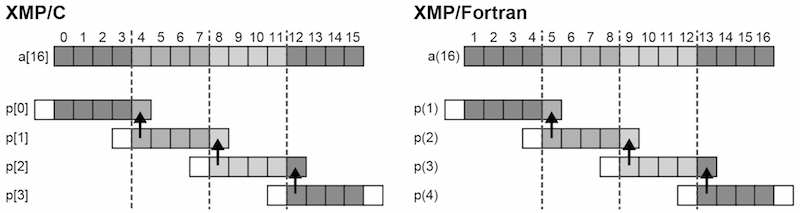
\includegraphics{figs/reflect_width.png}
\end{figure}

\begin{mynote}
If the widths of the shadow areas to be updated on
the upper and lower 
bounds are equal, that is, for example, width(1:1), you can abbreviate
it as width(1).
\end{mynote}

\begin{mynote}
It is not possible to update the shadow area on a
particular node. 
\end{mynote}

If no shadow area is specified on the lower bound, the reflect directive
does not update it with or without a width clause. The below figure
illustrates the behavior of a reflect directive for a distributed array
a having a shadow area of width one only on the upper bound.

\begin{figure}
  \centering
  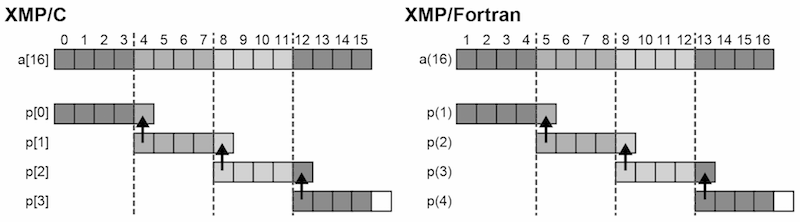
\includegraphics{figs/reflect_uneven.png}
\end{figure}

\paragraph{Update periodic shadow}

The reflect directive does not update either the shadow area on the
lower bound on the leading node or that on the upper bound on the last
node. However, the values in such areas are needed for stencil
computation if the computation needs a periodic boundary condition.

To update such areas, add a periodic qualifier into a width
clause. Let’s look at the following example where an array a having
shadow areas of width one on both the lower and upper bounds appears.

\begin{XCexample}
#pragma xmp reflect (a) width(/periodic/1:1)
\end{XCexample}

\begin{XFexample}
!$xmp reflect (a) width(/periodic/1:1)
\end{XFexample}

\begin{figure}
  \centering
  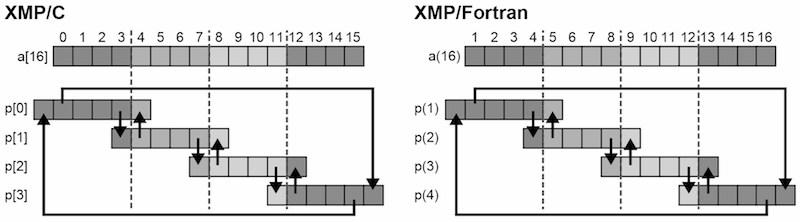
\includegraphics{figs/reflect_periodic.png}
\end{figure}

The periodic qualifier has the following effects, in addition to that of
a normal reflect directive: in XMP/C, node p[0] sends an element a[0] to
the shadow area on the upper bound on node p[3], and p[3] sends a[15] to
the shadow area on the lower bound on p[0]; in XMP/Fortran, node p(1)
sends an element a(1) to the shadow area on the upper bound on node
p(4), and p(4) sends a(16) to the shadow area on the lower bound on
p(1).

\begin{mynote}
If the widths of the shadow areas to be updated on
the upper and lower 
bounds are equal, as shown by width(/periodic/1:1) in the above example,
you can abbreviate it as width(/periodic/1).
\end{mynote}

\subsubsection{Multi-dimensional Shadow}

The shadow directive and reflect construct can be applied to distributed
arrays multiple dimensions. The following programs are the examples for
two-dimensional distribution.

\begin{XCexample}
#pragma xmp nodes p[3][3]
#pragma xmp template t[9][9]
#pragma xmp distribute t[block][block] onto p
double a[9][9];
#pragma xmp align a[i][j] with t[i][j]
#pragma xmp shadow a[1][1]
   :
#pragma xmp reflect (a)
\end{XCexample}

\begin{XFexample}
!$xmp nodes p(3,3)
!$xmp template t(9,9)
!$xmp distribute t(block,block) onto p
real :: a(9,9)
!$xmp align a(j,i) with t(j,i)
!$xmp shadow a(1,1)
   :
!$xmp reflect (a)
\end{XFexample}

\begin{figure}
  \centering
  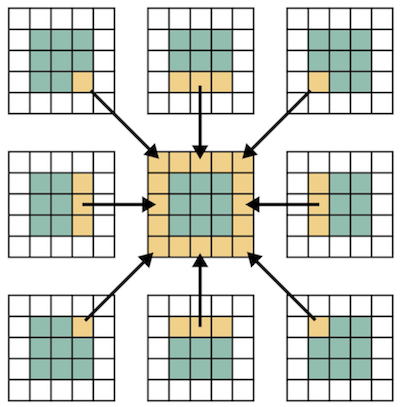
\includegraphics{figs/multi1.png}
\end{figure}

The central node receives the shadow data from the surrounding eight
nodes. The shadow areas of the other nodes are also updated, which is
omitted in the figure.

For some applications, data from ordinal directions are not
necessary. In such a case, the data communication from/to the ordinal
directions can be avoided by adding an orthogonal clause to a reflect
construct.

\begin{XCexample}
#pragma xmp reflect (a) orthogonal
\end{XCexample}

\begin{XFexample}
!$xmp reflect (a) orthogonal
\end{XFexample}

\begin{figure}
  \centering
  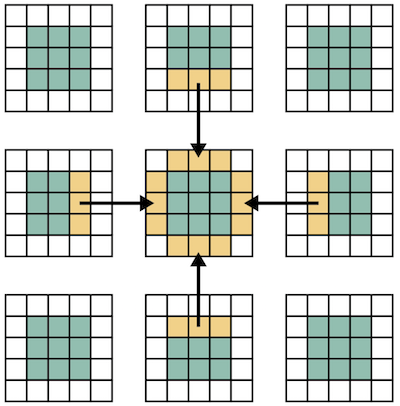
\includegraphics{figs/multi_orthogonal.png}
\end{figure}

\begin{mynote}
The orthogonal clause is effective only for arrays
more than one 
dimension of which is distributed.
\end{mynote}

Besides, you can also add shadow areas to only specified dimension.

\begin{XCexample}
#pragma xmp nodes p[3]
#pragma xmp template t[9]
#pragma xmp distribute t[block] onto p
double a[9][9];
#pragma xmp align a[i][*] with t[i]
#pragma xmp shadow a[1][0]
  :
#pragma xmp reflect (a)
\end{XCexample}

\begin{XFexample}
!$xmp nodes p[3]
!$xmp template t[9]
!$xmp distribute t[block] onto p
real :: a(9,9)
!$xmp align a(*,i) with t(i)
!$xmp shadow a(0,1)
  :
!$xmp reflect (a)
\end{XFexample}

\begin{figure}
  \centering
  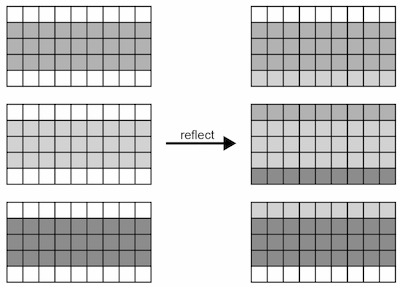
\includegraphics{figs/1of2.png}
\end{figure}

In the array specified in the shadow directive, 0 is set as the shadow
width in dimensions which are not distributed.


\subsection{{\tt gmove} Construct}

You can describe a communication for distributed arrays in the form of
assignment statements by using gmove directive.

There are three modes in gmove; “collective mode”, “in mode,” and “out
mode.” While collective mode executes two-sided communication among the
executing nodes, in/out modes execute one-sided communication among
tasks with a task directive. While in mode uses get communication, out
mode uses put communication.

\subsubsection{Collective Mode}

\paragraph{Distributed array}

Copying a part of array a to array b. Array assignment statements in a
gmove construct uses triplet.

\begin{XCexample}
#pragma xmp nodes p[4]
#pragma xmp template t[16]
#pragma xmp distribute t[block] onto p
int a[16], b[16];
#pragma xmp align a[i] with t[i]
#pragma xmp align b[i] with t[i]
     :
#pragma xmp gmove
  a[9:5] = b[0:5];
\end{XCexample}

\begin{XFexample}
!$xmp nodes p(4)
!$xmp template t(16)
!$xmp distribute t(block) onto p
integer :: a(16), b(16)
!$xmp align a(i) with t(i)
!$xmp align b(i) with t(i)
     :
!$xmp gmove
  a(10:14) = b(1:5)
\end{XFexample}

\begin{figure}
  \centering
  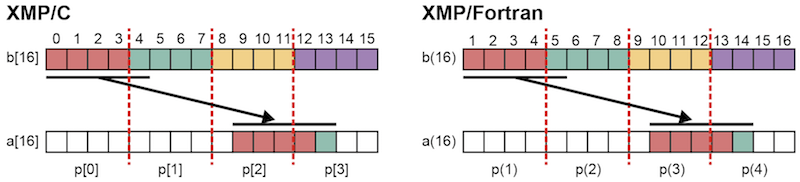
\includegraphics{figs/gmove.png}
\end{figure}

In XMP/C, p[0] sends b[0] - b[3] to p[2] - p[3], and p[1] sends b[4] to
p[3]. Similarly, in XMP/Fortran, p(1) sends b(1) - b(4) to p(3) - p(4),
and p(2) sends b(5) to p(4).

In this example, it is assignment statements between distributed arrays
with the same shape. XMP also supports to assign it with the different
shape.

\begin{XCexample}
#pragma xmp nodes p[4]
#pragma xmp template t1[16]
#pragma xmp template t2[16]
#pragma xmp distribute t1[cyclic] onto p
#pragma xmp distribute t2[block] onto p
int a[16], b[16];
#pragma xmp align a[i] with t1[i]
#pragma xmp align b[i] with t2[i]
     :
#pragma xmp gmove
  a[9:5] = b[0:5];
\end{XCexample}

\begin{XFexample}
!$xmp nodes p(4)
!$xmp template t1(16)
!$xmp template t2(16)
!$xmp distribute t1(cyclic) onto p
!$xmp distribute t2(block) onto p
integer :: a(16), b(16)
!$xmp align a(i) with t1(i)
!$xmp align b(i) with t2(i)
     :
!$xmp gmove
  a(10:14) = b(1:5)
\end{XFexample}

\begin{figure}
  \centering
  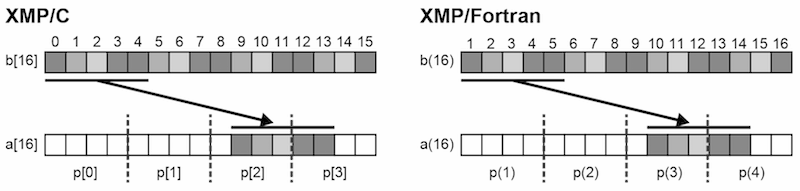
\includegraphics{figs/gmove_cyclic.png}
\end{figure}

While array a is distributed in a cyclic manner, array b is distributed
in a block manner.

In XMP/C, p[0] sends b[0] and b[4] to p[2] and p[3]. p[1] sends b[1] to
p[2]. Each element of p[2] and p[3] will be copied locally. Similarly,
in XMP/Fortran, p(1) sends b(1) and b(5) to p(3) and p(4). p(2) sends
b(2) to p(3). Each element of p(3) and p(4) will be copied locally.

\begin{mynote}
If the number of elements specified on the
right-hand side is other than one, it will not work properly if the
  number of elements differs between the right-hand side and the
  left-hand side.
\end{mynote}

By using this method, the shape of a distributed array can be changed
during calculation.

\begin{XCexample}
#pragma xmp nodes p[4]
#pragma xmp template t1[16]
#pragma xmp template t2[16]
int W[4] = {2,4,8,2};
#pragma xmp distribute t1[gblock(W)] onto p
#pragma xmp distribute t2[block] onto p
int a[16], b[16];
#pragma xmp align a[i] with t1[i]
#pragma xmp align b[i] with t2[i]
     :
#pragma xmp gmove
  a[:] = b[:];
\end{XCexample}

\begin{XFexample}
!$xmp nodes p(4)
!$xmp template t1(16)
!$xmp template t2(16)
integer :: W(4) = (/2,4,7,3/)
!$xmp distribute t1(gblock(W)) onto p
!$xmp distribute t2(block) onto p
integer :: a(16), b(16)
!$xmp align a(i) with t1(i)
!$xmp align b(i) with t2(i)
     :
!$xmp gmove
  a(:) = b(:)
\end{XFexample}

\begin{figure}
  \centering
  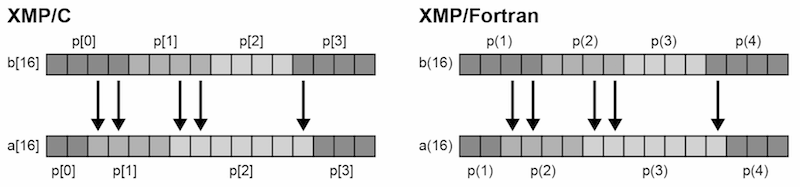
\includegraphics{figs/gmove_change.png}
\end{figure}

In this example, copying all elements of array b which is distributed in
a block manner to array a which is distributed in a gblock manner. In
arrays a and b, communication occurs only for elements whose responsible
nodes do not match (the arrow means communication between nodes in
figures).

\paragraph{Scalar}

In an assignment statement, if one element is specified on the
right-hand side and plural elements are specified on the left-hand side,
the operation will be broadcast communication.

\begin{XCexample}
#pragma xmp nodes p[4]
#pragma xmp template t[16]
#pragma xmp distribute t[block] onto p
int a[16], b[16];
#pragma xmp align a[i] with t[i]
#pragma xmp align b[i] with t[i]
     :
#pragma xmp gmove
  a[9:5] = b[0];
\end{XCexample}

\begin{XFexample}
!$xmp nodes p(4)
!$xmp template t(16)
!$xmp distribute t(block) onto p
integer :: a(16), b(16)
!$xmp align a(i) with t(i)
!$xmp align b(i) with t(i)
     :
!$xmp gmove
  a(10:14) = b(1)
\end{XFexample}

\begin{figure}
  \centering
  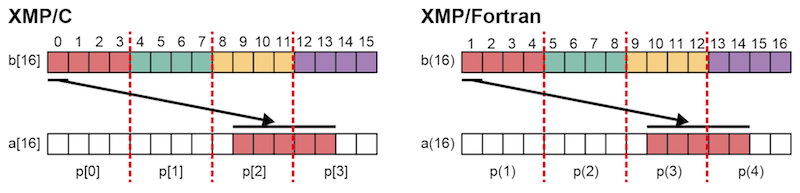
\includegraphics{figs/gmove_one_element.png}
\end{figure}

In this example, in XMP/C, an element array b[0] of node p[0] will be
broadcasted to the specified index of node p[2] and p[3]. Similarly, in
XMP/Fortran, an element array b(1) of node p(1) will be broadcasted to
the specified index of node p(3) and p(4).

\paragraph{Duplicated array and scalar}

Not only distributed arrays but also duplicated arrays and scalar
variables can be described on the right-hand side.

\begin{XCexample}
 #pragma xmp nodes p[4]
 #pragma xmp template t[16]
 #pragma xmp distribute t[block] onto p
 int a[16], b[16], c;
 #pragma xmp align a[i] with t[i]
      :
#pragma xmp gmove
   a[9:5] = b[0:5];

#pragma xmp gmove
   a[9:5] = c;
\end{XCexample}

\begin{XFexample}
 !$xmp nodes p(4)
 !$xmp template t(16)
 !$xmp distribute t(block) onto p
 integer :: a(16), b(16), c
 !$xmp align a(i) with t(i)
      :
!$xmp gmove
   a(10:14) = b(1:5)

!$xmp gmove
   a(10:14) = c
\end{XFexample}

In this example, duplicated array and scalar variable are copied to
distributed array locally. For this reason, communication does not
occur.

\paragraph{Distributed array with different dimension}

\begin{XCexample}
#pragma xmp nodes p[4]
#pragma xmp template t1[8]
#pragma xmp template t2[16]
#pragma xmp distribute t1[block] onto p
#pragma xmp distribute t2[block] onto p
int a[8][16], b[8][16];
#pragma xmp align a[i][*] with t1[i]
#pragma xmp align b[*][i] with t2[i]
     :
#pragma xmp gmove
  a[0][:] = b[0][:];
\end{XCexample}

\begin{XFexample}
!$xmp nodes p(4)
!$xmp template t1(8)
!$xmp template t2(16)
!$xmp distribute t1(block) onto p
!$xmp distribute t2(block) onto p
integer :: a(16,8), b(8,16)
!$xmp align a(*,i) with t1(i)
!$xmp align b(i,*) with t2(i)
     :
#pragma xmp gmove
  a(:,1) = b(:,1)
\end{XFexample}

\begin{figure}
  \centering
  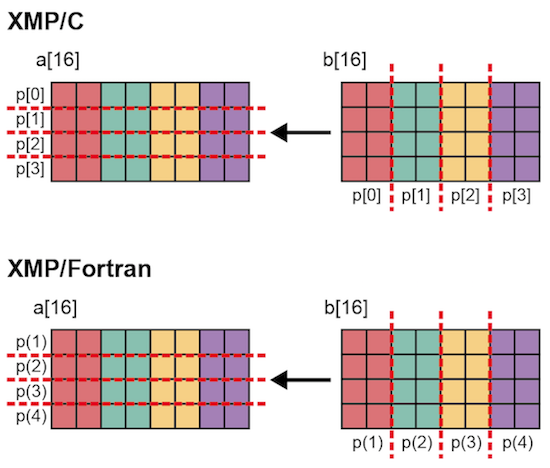
\includegraphics{figs/gmove_different.png}
\end{figure}

In this example, in XMP/C, b[0][0:2] of p[0], b[0][2:2] of p[1],
b[0][4:2] of p[2] and b[0][6:2] of p[3] are copied to a[0][:] of
p[0]. Similarly, in XMP/Fortran, b(1:2,1) of p(1), b(3:4,1) of p(2),
b(5:6,1) of p(3) and b(7:8,1) of p(4) are copied to a(:,1) of p(1).

\subsubsection{In Mode}

It operates as in mode by setting in clause to gmove directive.

\begin{XCexample}
#pragma xmp nodes p[4]
#pragma xmp template t[4]
#pragma xmp distribute t[block] onto p
double a[4], b[4];
#pragma xmp align a[i] with t[i]
#pragma xmp align b[i] with t[i]
   :
#pragma xmp task on p[0:2]
#pragma xmp gmove in
  a[0:2] = b[2:2]
#pragma xmp end task
\end{XCexample}

\begin{XFexample}
!$xmp nodes p(4)
!$xmp template t(4)
!$xmp distribute t(block) onto p
real :: a(4), b(4)
!$xmp align a(i) with t(i)
!$xmp align b(i) with t(i)
   :
!$xmp task on p(1:2)
!$xmp gmove in
  a(1:2) = b(3:4)
!$xmp end task
\end{XFexample}

In this example, the task directive divides the node set of 4 nodes into
two nodes, the first-half and the second-half. In gmove directive which
is in mode, it executes get communication from array of second-half node
to array of first-half node.

\begin{figure}
  \centering
  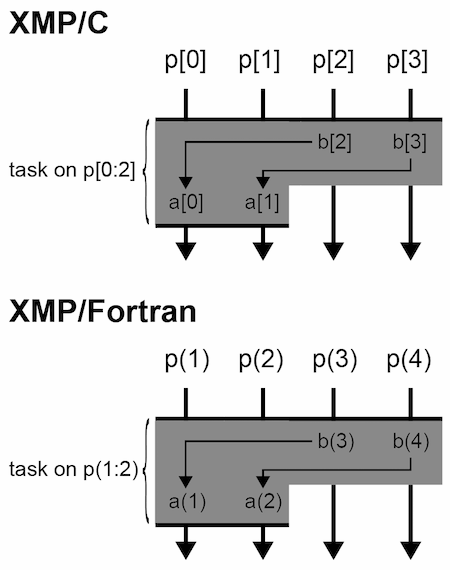
\includegraphics{figs/gmove_in.png}
\end{figure}


\subsubsection{Out Mode}

It operates as out mode by setting out clause to gmove directive

\begin{XCexample}
#pragma xmp nodes p[4]
#pragma xmp template t[4]
#pragma xmp distribute t[block] onto p
double a[4], b[4];
#pragma xmp align a[i] with t[i]
#pragma xmp align b[i] with t[i]
   :
#pragma xmp task on p[0:2]
#pragma xmp gmove out
  b[2:2] = a[0:2]
#pragma xmp end task
\end{XCexample}

\begin{XFexample}
!$xmp nodes p(4)
!$xmp template t(4)
!$xmp distribute t(block) onto p
real :: a(4), b(4)
!$xmp align a(i) with t(i)
!$xmp align b(i) with t(i)
   :
!$xmp task on p(1:2)
!$xmp gmove out
  b(3:4) = a(1:2)
!$xmp end task
\end{XFexample}

In this example, it just reversed the assignment statement of the in
mode. In gmove directive which is out mode, it executes put
communication from array of first-half node to array of second-half
node.

\begin{figure}
  \centering
  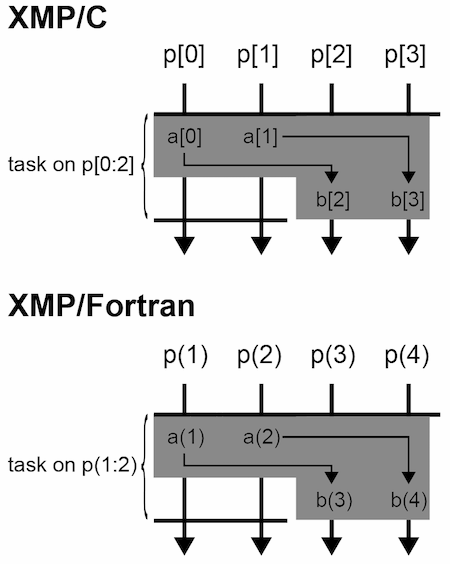
\includegraphics{figs/gmove_out.png}
\end{figure}


\subsection{{\bf barrier} Construct}

Execute barrier synchronization.

\begin{XCexample}
#pragma xmp barrier
\end{XCexample}

\begin{XFexample}
!$xmp barrier
\end{XFexample}

You can set the barrier range by using the on clause. In the below
example, barrier synchronization occurs only in the first two nodes of
p.

\begin{XCexample}
#pragma xmp barrier on p[0:2]
\end{XCexample}

\begin{XFexample}
!$xmp barrier on p(1:2)
\end{XFexample}


\subsection{{\bf reduction} Construct}

Execute reduction operation. It has the same meaning as the reduction
clause of loop construct, but the reduction directive can be described
anywhere.

\begin{XCexample}
#pragma xmp nodes p[4]
  :
sum = xmpc_node_num() + 1;
#pragma xmp reduction (+:sum)
\end{XCexample}

\begin{XFexample}
!$xmp nodes p(4)
  :
sum = xmp_node_num()
!$xmp reduction (+:sum)
\end{XFexample}

\begin{figure}
  \centering
  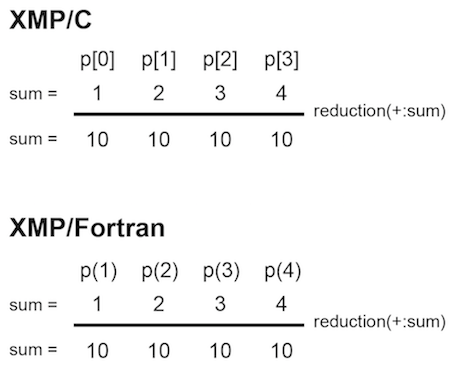
\includegraphics{figs/reduction.png}
\end{figure}

You can set the range of the node set by using the on clause. In the
below example, only the values of the last two nodes in four nodes are
targets to reduction operation.

\begin{XCexample}
#pragma xmp nodes p[4]
  :
sum = xmpc_node_num() + 1;
#pragma xmp reduction (+:sum) on p[2:2]
\end{XCexample}

\begin{XFexample}
!$xmp nodes p(4)
  :
 sum = xmp_node_num()
 !$xmp reduction (+:sum) on p(3:4)
\end{XFexample}

\begin{figure}
  \centering
  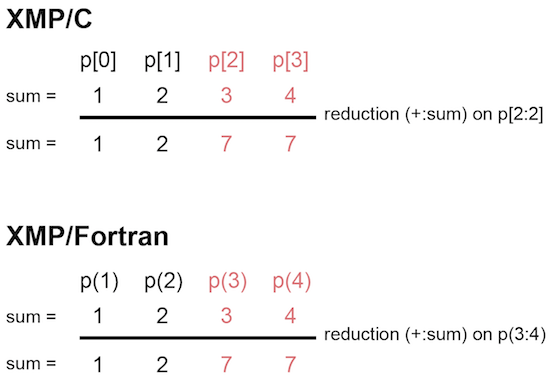
\includegraphics{figs/reduction_on.png}
\end{figure}

The specifiable operators are as follows.

\begin{XCexample}
+
*
-
&
|
^
&&
||
max
min
\end{XCexample}

\begin{XFexample}
+
*
-
.and.
.or.
.eqv.
.neqv.
max
min
iand
ior
ieor
\end{XFexample}

\begin{mynote}
Since the reduction clause needs a loop statement,
operators of
firstmax, firstmin, lastmax, and lastmin are required. But, since the
reduction directive does not need a loop statement, there are no such
operators.
\end{mynote}

\begin{mynote}
Similar to the reduction clause, the reduction
directive may have
slightly different results from sequential execution and parallel
execution, because of depending on the calculation order when the
reduction variable is a floating-point type.
\end{mynote}


\subsection{{\bf bcast} Construct}

The bcast directive broadcasts variables which are held by the node,
specified in the from clause, to the node set specified in the on
clause. If there is no from clause, the first node of the target node
set is the starting point. If there is no on clause, the current set of
nodes will be covered.

In the below example, the first node of the node set p is the starting point.

\begin{XCexample}
#pragma xmp nodes p[4]
  :
num = xmpc_node_num() + 1;
#pragma xmp bcast (num)
\end{XCexample}

\begin{XFexample}
!$xmp nodes p(4)
  :
num = xmp_node_num()
!$xmp bcast (num)
\end{XFexample}

\begin{figure}
  \centering
  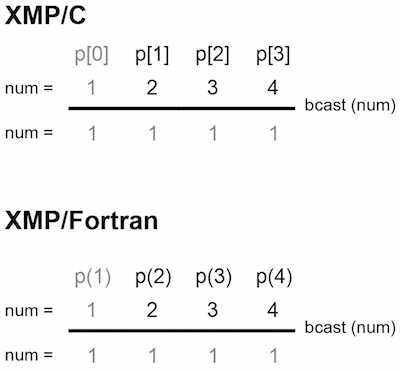
\includegraphics{figs/bcast.png}
\end{figure}

In the below example, starting from the last node of the node set p by
the from clause.

\begin{XCexample}
#pragma xmp nodes p[4]
  :
num = xmpc_node_num() + 1;
#pragma xmp bcast (num) from p[3]
\end{XCexample}

\begin{XFexample}
!$xmp nodes p(4)
  :
num = xmp_node_num()
!$xmp bcast (num) from p(4)
\end{XFexample}

\begin{figure}
  \centering
  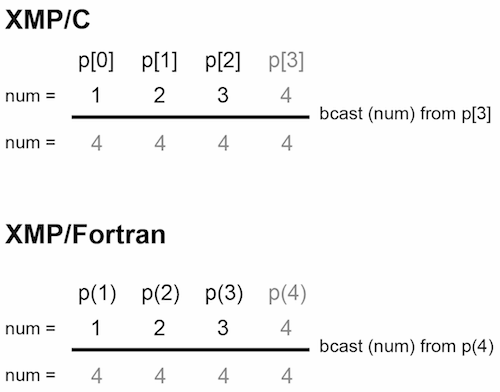
\includegraphics{figs/bcast_from.png}
\end{figure}

In the below example, only the values of the last three nodes in 4 nodes
are targets for communication by the on clause.

\begin{XCexample}
#pragma xmp nodes p[4]
  :
sum = xmpc_node_num() + 1;
#pragma xmp bcast (num) from p[3] on p[1:3]
\end{XCexample}

\begin{XFexample}
!$xmp nodes p(4)
  :
 sum = xmp_node_num()
 !$xmp bcast (num) from p(4) on p(2:4)
\end{XFexample}

\begin{figure}
  \centering
  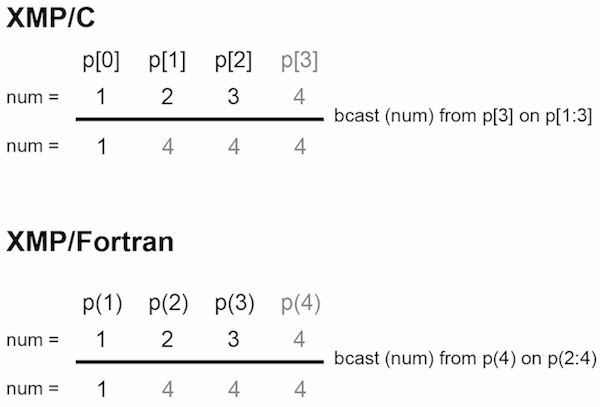
\includegraphics{figs/bcast_from_on.png}
\end{figure}


\subsection{{\bf wait\_async} Construct}

Communication directives (reflect, gmove, reduction, bcast,
reduce\_shadow) can execute asynchronous communication by attaching the
“async” clause. The wait\_async directive is used to guarantee the
completion of their asynchronous communication.

\begin{XCexample}
#pragma xmp bcast (num) async(1)
    :
#pragma xmp wait_async (1)
\end{XCexample}

\begin{XFexample}
!$xmp bcast (num) async(1)
        :
!$xmp wait_async (1)
\end{XFexample}

Since the bcast directive has an async clause, communication may not be
completed immediately after the bcast directive. Completion of that
communication is guaranteed with the wait\_async directive whose the same
value as the async clause is specified. Therefore, between the bcast
directive and the wait\_async directive, you can not operate on the
variable specified in the bcast directive.

\begin{myhint}
By performing calculations without a dependency
relationship with the variable specified by the bcast directive after
the bcast directive, overlap of communication and calculation can be
performed, so the total calculation time may be small.
\end{myhint}

\begin{mynote}
Values that can be specified for async clause are
int type in XMP/C, and
integer type in XMP/Fortran.
\end{mynote}

\subsection{{\bf reduce\_shadow} Construct}

The reduce\_shadow directive adds the value of the shadow to the value of
the source element.

\begin{XCexample}
#pragma xmp nodes p[2]
#pragma xmp template t[8]
#pragma xmp distribute t[block] onto p
int a[8];
#pragma xmp align a[i] with t[i]
#pragma xmp shadow a[1]
 :
#pragma xmp loop on t[i]
  for(int i=0;i<8;i++)
    a[i] = i+1;

#pragma xmp reflect (a)
#pragma xmp reduce_shadow (a)
\end{XCexample}

\begin{XFexample}
!$xmp nodes p(2)
!$xmp template t(8)
!$xmp distribute t(block) onto p
  integer a(8)
!$xmp align a(i) with t(i)
!$xmp shadow a(1)

!$xmp loop on t(i)
  do i=1, 8
    a(i) = i
  enddo

!$xmp reflect (a)
!$xmp reduce_shadow (a)
\end{XFexample}

The shadow directive adds one shadow to the distributed array a of each
node. Next, the reflect directive will update shadow between
neighborhood nodes. Finally, the reduce\_shadow directive adds the value
of the shadow to the value of the source element.

In XMP/C, a[3] of p[0] has a value of 8, and a[4] of p[1] has a value of
10. Similarly, in XMP/Fortran, a(4) of p(1) has a value of 8, and a(5)
of p(2) has a value of 10.

\begin{figure}
  \centering
  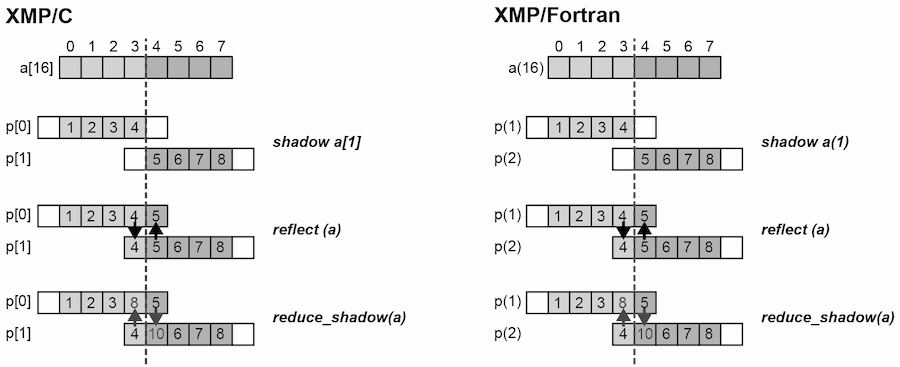
\includegraphics{figs/reduce_shadow.png}
\end{figure}

You can add the periodic modifier to the width clause to execute
periodic region updates.

\begin{XCexample}
#pragma xmp reflect (a) width(/periodic/1)
#pragma xmp reduce_shadow (a) width(/periodic/1)
\end{XCexample}

\begin{XFexample}
!$xmp reflect (a) width(/periodic/1)
!$xmp reduce_shadow (a) width(/periodic/1)
\end{XFexample}

\begin{figure}
  \centering
  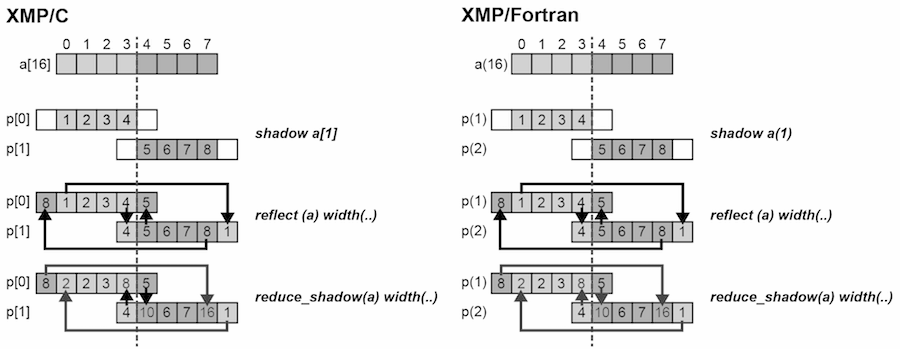
\includegraphics{figs/reduce_shadow_periodic.png}
\end{figure}

In addition to the first example, in XMP/C, a[0] of p[0] has a value of
2, and a[7] of p[1] has a value of 16. Similarly, in XMP/Fortran, a(1)
in p(1) has a value of 2, and a(8) in p(2) has a value of 16.